\documentclass[coguia]{tesis-usach}
% Opciones: coguia, propuesta

\begin{document}
\baselineskip 23pt
\frontmatter								% Utiliza numeración romana

% ### Cubierta de la tesis ###
\thispagestyle{empty}
\facultad{Ingeniería}
\departamento{Ingeniería Informática}
\grado{Grado}

\titulo{Análisis de sentimientos basado en minería de texto de la serie de libros Papelucho.}

\autor{Sebastián Ignacio Villalobos Pérez}
\email{sebastian.villalobos.p@usach.cl}
\run{16609266-3}		% S\'olo necesario en propuesta
\telefono{22222222}		% S\'olo necesario en propuesta
\annoingreso{2017}

\fecha{Viernes}{22}{Octubre}{2021}

\profesorguia{Manuel Villalobos Cid}

\ciudad{Santiago}
\pais{Chile}

\makecubierta


% ### Páginas preliminares de la tesis ###
\pagestyle{fancy}
\renewcommand{\headrulewidth}{0pt}		% Hace que no aparezca la línea horizontal superior al principio de estas páginas
\fancyhead[L]{}
\fancyhead[C]{}
\fancyhead[R]{}

{\setstretch{1.0}						% Interlineado en las páginas https://www.overleaf.com/project/6172d071ced6744d4682d6ddpreliminares
%\makecopyright			 comentado				% Si es propuesta no se mostrará

% ### Resumen de la tesis
%\setcounter{page}{0} 
%\resumenCastellano{

Como en cualquier tipo de competición, el objetivo principal es ganar y el videojuego de estrategia en tiempo real, StarCraft II, no es la excepción. Uno de los aspectos más importantes, en el ámbito competitivo de este juego, son los órdenes de construcción, que consisten en patrones de juego para guiar al jugador hasta una unidad o estructura deseada, cuya importancia radica en qué tan buenos son en contraste con los que utilicen los oponentes, dejando al jugador que posea el mejor orden de construcción con una ventaja en su estrategia respecto al contrincante. En esta investigación se detalla un modelo propuesto basado en la metaheurística \textit{Simulated Annealing} que permite obtener órdenes de construcción al nivel de los usados por profesionales del videojuego al optimizar el tiempo de partida que estas secuencias requieren para alcanzar una unidad, un edificio o una mejora de la raza Terran.

\vspace*{0.5cm}
\KeywordsES{StarCraft II, metaheurísticas, optimización, RCPSP, simulated annealing}
}

\newpage


% ### Dedicatoria y agredecimientos de la tesis ###
%\dedicatoria{
Even if your births and backgrounds are unknown,\\
and you don't have a master to serve or a sword to fight,\\
you can each carry your own bushido in your hearts\\
and become your own samurai.
}
		% En caso de no querer agregarlos, comente esta línea
%\begin{agradecimiento}
Agradezco inmensamente a mi familia, principalmente a mi madre que siempre está preocupándose por mí y apoyándome en todo lo que puede. También a mi hermana que me escuchaba pacientemente cada vez que algo salía mal, aún si no entendía del todo lo que intentaba explicarle. A mis primos que me ayudaban a despejar la mente jugando diversos videojuegos cuando les era posible. Tampoco puedo olvidar a mi perrito que me hizo compañía todas las noches que me tocaba quedarme hasta la madrugada.

Además, le agradezco a mi profesor guía, Manuel Villalobos Cid, por su constante apoyo durante el avance de este proyecto, pues me enseñó con mucha paciencia muchos conceptos interesantes que desconocía antes de comenzar, además de siempre hacerse un tiempo cuando tenía dudas, sin importar si era horario de almuerzo o un fin de semana en la noche. También a mis compañeros bajo el ala del profesor, principalmente a Brandon y a Andrés que vivieron el proceso de la tesis junto a mí.

Finalmente, quiero agradecer a mis amigos que conocí en la universidad, quienes, durante todos estos años, rieron conmigo en los momentos buenos y sufrieron conmigo en los difíciles. Sin ellos, definitivamente no podría haber llegado hasta acá, así que les agradezco con toda el alma.

\end{agradecimiento}

% ### Índices ###
\tableofcontents							%% Tabla de contenido

%\listoftables							%% Indice de tablas
%\listoffigures							%% Indice de figuras
%\listofalgorithms
%\AtBeginEnvironment{algorithmic}{\setstretch{1.5}} % Interlineado de los algoritmos
} % end \setstretch{1.0}

% ### Cuerpo de la tesis ###
\mainmatter								% Reinicia el contador de páginas para partir de 1 y usando números arábicos.

% ### Capítulos de la tesis ###
% caption source
\newcommand*{\captionsource}[1]{%
 \caption[{#1}]{%
 #1%
 \\\hspace{\linewidth}%
 \textbf{Fuente:} Elaboración propia, 2021%
 }%
}

\newcommand*{\captionimg}[2]{%
 \caption[{#1}]{%
 #1%
 \\\hspace{\linewidth}%
 \textbf{Fuente:} #2%
 }%
}


\chapter{Introducci\'on}
\label{cap:introduccion}

\section{Antecedentes y motivaci\'on}
\label{intro:motivacion}
StarCraft II es un videojuego de estrategia en tiempo real (RTS por sus siglas en inglés) desarrollado por Blizzard Entertainment donde cada jugador escoge una de las tres razas (Terran, Protoss y Zerg) por partida, de las cuales, cada una tiene características particulares en términos de funcionamiento, unidades y tecnologías en comparación con las otras dos, lo que resulta en una jugabilidad o experiencia de juego distinta para cada raza. En el caso de los Terran, una especie basada en humanos con tecnologías futuristas, su modo de juego gira en torno a la movilidad de sus unidades para intervenir con las bases enemigas en distintos puntos a la vez, siendo el posicionamiento uno de los puntos clave a la hora de usarles.

Aunque puede parecer un tema banal, los videojuegos de estrategia en tiempo real tienen aplicaciones fuera del ámbito de la entretención. En la medicina se sugiere que los videojuegos RTS ayudan a mejorar las habilidades cognitivas de sus jugadores  (Glass, Maddox, \& Love, 2013) al necesitar la atención simultánea en múltiples aspectos dentro del juego. Existe también, en el área educacional el caso de StarCraft II siendo utilizado como herramienta seria para enseñar, no sólo teoría de videojuegos, sino que también, matemáticas avanzadas y conceptos economía (Kuo, 2012).

Si bien es sabido que en cualquier juego competitivo el objetivo es intentar ganar al oponente, no siempre resulta sencillo lograrlo, por lo que es lógico buscar otros acercamientos que nos entreguen nuevas metodologías o estrategias que sean mejores y más eficientes que las ya existentes de manera que se pueda estar, aunque sea solo un paso, por delante del rival con la finalidad de obtener la victoria por sobre este ya sea en un videojuego o, incluso, en un deporte. Dicho esto, en el ámbito de las competencias profesionales de videojuegos (también conocidos como \textit{esports}), StarCraft II posee actualmente dos organizadores oficiales (ESL y DreamHack) cuyas competiciones poseen premios de hasta 500.000 dólares.

Al tomar en cuenta los métodos que utilizan los jugadores de StarCraft II para mejorar, se encuentran dos focos principales: aprender de las repeticiones que ofrece el juego y el \textit{theorycrafting} (Kow \& Young, 2013). Este último involucra la búsqueda de información acerca del juego a través de medios que son, en gran parte, no oficiales y que van desde videos explicativos hasta foros en línea y \textit{wikis}, conteniendo, en su mayoría, estrategias y debates por parte de los mismos jugadores, siendo de utilidad, sobre todo, para aquellos con pocos conocimientos sobre optimización. Aún si puede parecer sencillo mejorar en el juego siguiendo estos medios, nada asegura que la información obtenida sea de ayuda, pues quienes redactan o participan en la creación de esta no siempre son jugadores profesionales o competentes en el juego. 

Debido a que existen un sinfín de factores que afectan el resultado de una partida de StarCraft II, como el manejo de recursos, el posicionamiento o las decisiones inmediatas y a futuro de los jugadores, es que el intentar optimizar los órdenes de construcción (secuencias que indican las unidades que deben ser creadas en un tiempo determinado), que cambian constantemente durante una partida, en reacción a muchos factores como los mencionados anteriormente, se considera un problema de complejidad \textit{NP-Hard} al igual que algunos de los juegos más conocidos de Nintendo como Super Mario o Pokémon (Aloupis, Demaine, Guo, \& Viglietta, 2012). 

Ante esto se tiene que la búsqueda de órdenes de construcción no puede ser abordada para encontrar un óptimo en un tiempo razonable, por lo que de ahora en adelante se referirán como “buenos órdenes de construcción” aquellos órdenes de construcción que sean utilizados por jugadores profesionales o competitivos de alto rango (dígase de aquellos con rango Maestro o Gran Maestro dentro del \textit{ranking} de clasificación del juego), además de aquellas que logren mejorar uno o más de los elementos que estos involucran, sean tiempo de la partida, cantidad de unidades, cantidad de estructuras o cantidad de recursos, cuya importancia varía dependiendo de la estrategia de los jugadores.

\section{Estado del arte}

En la actualidad, existen diversos trabajos relacionados con este género de videojuegos bajo distintos enfoques y con aplicaciones diferentes. Gran parte enfocados en el desarrollo de inteligencias artificiales para competencias entre estas mismas y de las estrategias y algoritmos que estas inteligencias artificiales requieren para lograr la victoria.

Aunque en el país no existen investigaciones al respecto, internacionalmente se pueden encontrar muchos trabajos en torno a StarCraft, el primer juego de la saga del mismo nombre lanzado en 1998, o a otros juegos de estrategia en tiempo real.

Si bien, ya hace 10 años que StarCraft II fue lanzado al mercado, en la actualidad siguen apareciendo nuevos trabajos enfocados sobre su precuela, StarCraft, ya que ambos son catalogados como \textit{benchmarks} importantes en cuanto a investigación de inteligencia artificial se refiere (Wang L. , Zeng, Chen, Pan, \& Cao, 2020). Con la finalidad de obtener la victoria, es que surgen investigaciones que atacan distintos puntos del juego en la búsqueda de algoritmos o metodologías que ayuden a estas inteligencias artificiales y, en algunos casos, a los jugadores humanos. En los enfoques estudiados se encuentran el uso de \textit{Machine Learning} en una inteligencia artificial que tras perfeccionarse a través de diversos tipos de aprendizaje logró llegar a altos rangos en la tabla de clasificación de StarCraft II al quedar por sobre el 99,8\% de los jugadores (Vinyals, y otros, 2019); el análisis de datos de repeticiones publicadas por Blizzard Entertainment con el fin de encontrar órdenes de construcción óptimas en StarCraft luego de comparar un acercamiento dirigido por datos con un acercamiento tradicional, ambos bajo el enfoque de un algoritmo genético y probados en enfrentamientos entre Terran contra Terran, llegando a la conclusión de que el primer acercamiento obtenía mejores resultados que uno tradicional (Wang P. , Zeng, Chen, \& Cao, 2019); o la evaluación de la efectividad de un conjunto de unidades frente a otro utilizando \textit{fuzzy integrals} en un algoritmo genético particular al comparar la precisión con que el algoritmo acierta el grupo de unidades vencedor de miles de enfrentamientos en un simulador, aunque el algoritmo falla al no tomar en cuenta algunos elementos del juego (Wang L. , Zeng, Chen, Pan, \& Cao, 2020).

Actualmente, no existe una solución que permita encontrar buenos órdenes de construcción en StarCraft II para llegar a una unidad especificada por un jugador humano, aunque hay investigaciones de hace algunos años que buscan que inteligencias artificiales logren decidir cuál de los órdenes de construcción preestablecidos usar según la información obtenida del enemigo en la partida, esto al trabajar con la inteligencia artificial de libre acceso \textit{UAlbertaBot} e integrarle un algoritmo de selección de órdenes de construcción que tiene en cuenta la información actual de la partida, cuyo resultado fue una mejora en la inteligencia artificial mencionada, logrando derrotar a la inteligencia artificial del juego un 91,7\% de las partidas, pero sin ser muy eficaz ante estrategias de ataque temprano o \textit{rush} (Justesen \& Risi, 2017) y otras que entregan un análisis al usuario acerca del mejor orden de construcción según la cantidad de recursos en base a órdenes de construcción predeterminados, esto fue probado al aplicar el algoritmo (una versión modificada del NSGA II) a las tres razas y simular una partida de 450 segundos, llegando a la conclusión de que esta herramienta resulta útil para que los jugadores mejoren sus estrategias (Köstler \& Gmeiner, 2013). Trabajos más antiguos también buscan la predicción de las estrategias de los oponentes con la información recopilada por una unidad que explore el escenario en busca del enemigo. Esto aplicado en una inteligencia artificial (Park, Lee, Cho, \& Kim, 2012) e, incluso, la creación automática de escenarios para el juego (Togelius, y otros, 2010).

A través de esta revisión sistemática se puede observar que gran parte de la investigación en torno al juego se aplica en las inteligencias artificiales que compiten entre ellas, dejando a los jugadores humanos en segundo plano y sin muchas soluciones que les ayuden a obtener la victoria o aumenten sus posibilidades de juego. Esto sin contar las escasas opciones que les entrega el juego mismo, las cuales se pueden reducir a un tutorial muy básico para aprender las mecánicas necesarias y la campaña individual con situaciones de juego preestablecidas. Estos antecedentes dejan a un jugador, con intenciones de mejorar, la única opción de aprender por su cuenta al observar a profesionales o aprender de la experiencia al jugar en línea contra otros oponentes en sus mismas condiciones.

Es importante tener en mente que todos los acercamientos mencionados para StarCraft II en esta sección son anticuados dado que, al igual que muchos videojuegos competitivos en línea, existen parches obligatorios que son lanzados con distinta frecuencia cuyo objetivo principal es modificar el videojuego para equilibrar los aspectos del mismo (debilitando personajes muy fuertes o mejorando los más débiles), como también solucionar errores o agregar nuevas funcionalidades. Con esto, se hace relevante informar que en la actualidad Blizzard ha cesado de lanzar nuevos parches de actualización para StarCraft II.

\section{Descripci\'on del problema}
\label{intro:problema}
Dada la contextualización anterior y como no existe una metodología o un camino feliz con el que encontrar buenos órdenes de construcción, es que los jugadores no pueden mejorar sus estrategias sin dedicar algo de su tiempo en la búsqueda de órdenes de construcción. Por esto, surge la pregunta: \textbf{¿cómo encontrar órdenes de construcción de forma más eficiente que un orden de construcción aleatorio y en un tiempo razonable, que permitan conseguir una unidad, estructura o tecnología determinada para la raza Terran en StarCraft II?}

\section{Objetivos del proyecto}
\label{intro:objetivos}

\subsection{Objetivo general}

Desarrollar un modelo, bajo un marco del algoritmo metaheurístico \textit{simulated annealing}, que permita generar buenos órdenes de construcción en el videojuego StarCraft II para la raza Terran, optimizados con el criterio del tiempo que requieren estas secuencias para llegar a la unidad, estructura o tecnología deseada.

\subsection{Objetivos específicos}

\begin{enumerate}
\item Modelar el árbol de tecnologías de la raza Terran con sus características y requisitos necesarios para la aplicación del algoritmo.

\item Modelar los elementos del juego StarCraft II necesarios para la aplicación del algoritmo.

\item Implementar SA para la obtención de buenos órdenes de construcción.

\item Evaluar los resultados del algoritmo implementado según el criterio del tiempo.
\end{enumerate}

% Please add the following required packages to your document preamble:
% \usepackage{multirow}
% \usepackage{graphicx}

\section{Metodología}
Si bien se contempla un componente de desarrollo que acompañe al algoritmo obtenido, el foco del presente proyecto se encuentra en la investigación. Ante esto es que se propone trabajar bajo el marco de una metodología por etapas (Villalobos-Cid, y otros, 2020) con el método científico como base. Revisados los objetivos del proyecto y las características de la solución es que se proponen tres etapas para el desarrollo del modelo. La primera etapa consta de la representación computacional de la raza Terran y la información del juego. La segunda etapa trata de la aplicación de un algoritmo metaheurístico a fin de obtener las soluciones. En la tercera etapa se evalúan los resultados obtenidos de la etapa anterior. Transversalmente a esas tres etapas, se aplicará una etapa de documentación en dónde se redacta el informe correspondiente con la información pertinente al proyecto.

\subsection{Etapa 1: Representaci\'on}

Engloba los objetivos específicos 1 y 2. En esta etapa se buscan representar computacionalmente los datos del juego necesarios para la aplicación del algoritmo simulated annealing, incluyendo los requisitos y características de las unidades, tecnologías y estructuras como indica el árbol de tecnologías, además de otros elementos, como la cantidad de recursos obtenidos en el tiempo, que influyen fuertemente en los órdenes de construcción.

\subsection{Etapa 2: Implementaci\'on}

Alineada con el objetivo específico 3, esta etapa tiene como propósito la aplicación de SA al utilizar la representación del paso anterior, además de los parámetros que deben ser definidos para uso del mismo algoritmo (temperatura inicial, probabilidad de aceptación, etc.). Para lograr esta implementación es que en esta fase se debe programar el algoritmo y ejecutarlo, obteniendo así los órdenes de construcción resultantes.

\subsection{Etapa 3: Evaluaci\'on}

Etapa que se asocia con el objetivo específico 4. En esta se evaluarán los resultados obtenidos de la implementación del algoritmo metaheurístico según el tiempo, comparándolo con los órdenes de construcción que sean utilizados por jugadores profesionales y jugadores competitivos (según sus rangos) de StarCraft II.

También se contempla la evaluación del SA al comparar los resultados entre sí, ya sea para las mismas o distintas entradas, para así analizar el comportamiento del algoritmo en cuanto a la calidad de sus soluciones o al tiempo que tarda en ejecutarse.

\subsection{Etapa de documentación}

Esta etapa, que va paralela a las tres anteriores, involucra todos los objetivos específicos, pues es necesaria para evidenciar por completo los procesos y resultados del proyecto.

\section{Ambiente de desarrollo y herramientas}

\subsection{Ambiente de ejecución}

A lo largo del proyecto se trabajará sobre un Notebook Asus modelo X556U, con un procesador Intel Core i5-7200U (2.5 GHz x4), memoria RAM de 8 GB, disco duro de 1 TB y una tarjeta gráfica integrada Intel HD Graphics 620. Todo esto con un sistema operativo Ubuntu 20.04.1 LTS.

\subsection{Herramientas}

Durante el desarrollo de la solución es necesaria la utilización de las siguientes herramientas: 
\begin{itemize}
\item R: lenguaje de programación especializado para la programación estadística. Será utilizado para implementar la solución propuesta. 
\item Visual Studio Code: editor de texto que destaca la sintaxis específica de cada lenguaje. Será el editor en el que se codificará. 
\item GitLab: herramienta de gestión de código fuente. Será utilizado como control de versiones del código. 
\item Microsoft Word: herramienta de procesamiento de textos. Será utilizado para redactar el informe.
\end{itemize}

\section{Alcance y limitaciones}

A continuación, se indican los alcances y limitaciones a los que está sujeta la solución propuesta.

\begin{itemize}
 \item El algoritmo metaheurístico encuentra órdenes de construcción que apliquen sólo para la raza Terran del juego StarCraft II, por lo que su aplicación a otras razas del mismo juego o a otros videojuegos escapa del alcance propuesto en este proyecto.

 \item La interfaz que se incluye en el proyecto tiene el único propósito de probar el algoritmo y sus resultados, por lo que no se espera aplicar ningún tipo de métricas de usabilidad ni la inclusión de un manual de usuario que facilite su uso.

 \item El programa será desarrollado en R.

 \item El modelo no tomará en cuenta elementos del juego como posicionamiento, unidades o estructuras perdidas, el tipo de escenario o cualquier elemento que involucre al oponente. Además, se asume que el jugador siempre tiene acceso a la extracción de recursos.
\end{itemize}

Con esto en cuenta, para la evaluación de la solución se compararán el tiempo de la partida en los órdenes de construcción generados para obtener una unidad, estructura o tecnología específica con los utilizados por jugadores profesionales y competitivos según los datos de repeticiones obtenidos de diversos repositorios, como los listados en https://liquipedia.net/starcraft2/Replay\_Websites, a modo de analizar si el modelo provee mejores órdenes de construcción que los jugadores competitivos en los distintos rangos del ranking o que un jugador profesional.

También se evaluará la eficiencia del algoritmo SA según el tiempo de ejecución que tarde para encontrar una solución, además de la convergencia de las generaciones. Todo esto para distintas entidades.


\section{Estructura del Documento}

En cuanto al formato de este documento, obviando las secciones de este Capítulo de introducción, se tiene el marco teórico que presenta definiciones del videojuego StarCraft II y de la metaheurística \textit{Simulated Annealing}, pues son utilizadas en el resto del presente documento. Continúa el estado del arte que indica los acercamientos existentes para el problema u otros trabajos relacionados al videojuego de estrategia en tiempo real. Sigue la especificación del algoritmo propuesto, dónde se detallan los elementos que este contiene. El quinto Capítulo de los experimentos con sus resultados explica los pasos realizados con el algoritmo y los efectos que surgieron de ellos. Después se analizan estos resultados en el Capítulo 6, indicando como fue el comportamiento de estos. El último Capítulo del cuerpo del documento trata de las conclusiones, haciendo una retrospectiva con todos los elementos vistos hasta el momento. Luego vienen el Glosario con algunos de los términos más importantes y las referencias a los trabajos externos revisados en este documento.


\chapter{Marco Teórico}

Antes de avanzar en los capítulos de este documento, es de vital importancia aclarar los conceptos utilizados de modo que exista una base de conocimiento que permita la total comprensión de los temas tratados.

\section{StarCraft II}

No todos los videojuegos son iguales y StarCraft II no es una excepción, por lo que detallar algunos de sus términos es de gran utilidad para la comprensión del documento.

\subsection{Características generales}

Similar a otros juegos del género de estrategia en tiempo real, StarCraft II consiste principalmente de construir un \textbf{ejército} al gestionar los distintos recursos no renovables que existen en el campo de batalla (o \textbf{mapa} de ahora en adelante) con la finalidad de vencer al ejército rival. Todo esto sin turnos establecidos como en otros tipos de juegos de estrategia, pues al tratarse de un juego en tiempo real cada segundo desaprovechado solamente beneficia al oponente y su creciente ejército. Conociendo ya este objetivo de vencer al ejército del oponente, se puede decir que la victoria en una partida se obtiene al derrotar a todas las fuerzas que componen a dicho ejército o cuando el oponente, por voluntad propia, decide rendirse antes de que caiga su ejército.

Antes de iniciar una partida de StarCraft II, cada jugador debe escoger una de las tres \textbf{razas} existentes en el videojuego, las cuales poseen elementos muy distintos entre ellas, pero que se rigen bajo las mismas reglas. Como el documento se basa en la raza Terran, las definiciones y los ejemplos presentados en los capítulos que proceden se enfocan en la raza Terran, aún cuando muchos de estos términos aplican también a las razas Protoss y Zerg.

Una vez iniciado el juego, cada jugador recibe los elementos básicos para comenzar la creación de su ejército: doce trabajadores (\textit{SCV} en el caso de la raza Terran) y un edificio principal (\textit{Command Center} para la raza Terran). A partir de aquí, el jugador tiene libre albedrío para construir su ejército o atacar a las fuerzas enemigas.

\subsection{Árbol de tecnologías}

Si bien existen distintos tipos de entidades que componen la milicia de un jugador, el videojuego los divide en tres categorías que engloban las características de estos: unidades, edificios y mejoras. Aunque existen fuertes similitudes entre todas estas categorías, como el hecho de que todos poseen \textbf{requisitos} de alguna índole, sus funciones principales son muy distintas entre sí.

Las \textbf{unidades} son todas aquellas entidades que son producidas por algún edificio. Su papel consiste, principalmente, en ser la fuerza de ataque de un ejército al movilizarse por el mapa, aunque sus funciones no se limitan sólo a atacar, pues también existen unidades conocidas como \textbf{trabajadores} (que en el caso de la raza Terran reciben el nombre de \textit{SCV} o \textit{Space Construction Vehicles}) los cuales se encargan de la recolección de recursos y también de la construcción de edificios. Al tratarse de entidades que pueden participar en combate, existen \textbf{estadísticas} (como salud, armadura o ataque) asignadas a cada tipo de unidad.

Los \textbf{edificios} son estructuras construidas por los trabajadores o evolucionadas de otros edificios, que se encuentran generalmente fijados a una posición en el mapa (escogida por el jugador al momento de su creación). Su función primordial consiste en la creación de las distintas unidades, aunque su utilidad no se detiene ahí, ya que algunos edificios también poseen características defensivas, otros permiten la investigación de mejoras e incluso uno que aumenta la cantidad de \textbf{suministros} (necesarios para la producción de unidades). De igual manera que las unidades, los edificios poseen estadísticas ya que pueden ser destruidos, aunque sólo algunos tienen estadísticas de ataque.

Tal como indica su nombre, las \textbf{mejoras} ofrecen distintos tipos de beneficios al resto de entidades, los cuales van desde aumentos en sus estadísticas (como aumentos en el ataque o la defensa) hasta el desbloqueo de \textbf{habilidades} que sólo pueden usar unidades o edificios específicos. A diferencia de las unidades o los edificios, las mejoras sólo permiten la creación de una de cada mejora por partida. Como ejemplo se tiene que sólo se puede construir un \textit{Infantry Weapons Level 1} (mejora Terran) a la vez que puedes tener 10 o 15 \textit{Marines} (unidad Terran).

A causa de que a lo largo de este documento se suelen englobar estas tres categorías, es que a partir de ahora se referirá a las unidades, a los edificios y a las mejoras (tanto en conjunto como individualmente) cómo \textbf{entidades}.

Entendiendo las tres categorías de entidades, es que ahora se puede definir al \textbf{árbol de tecnologías} como las relaciones que tiene cada entidad con respecto al resto, el cual nos muestra los \textbf{requisitos} para desbloquear cada entidad (entidades que se necesitan antes de que la unidad en cuestión pueda ser creada) y su \textbf{entidad de creación} (entidad que se encarga de la creación de la entidad en cuestión, que en algunas ocasiones se transforma en esta entidad) tal como se puede observar en la {\ref{fig:2}}.

\begin{figure}[H]
	\centering
	\captionsetup{justification=centering}
	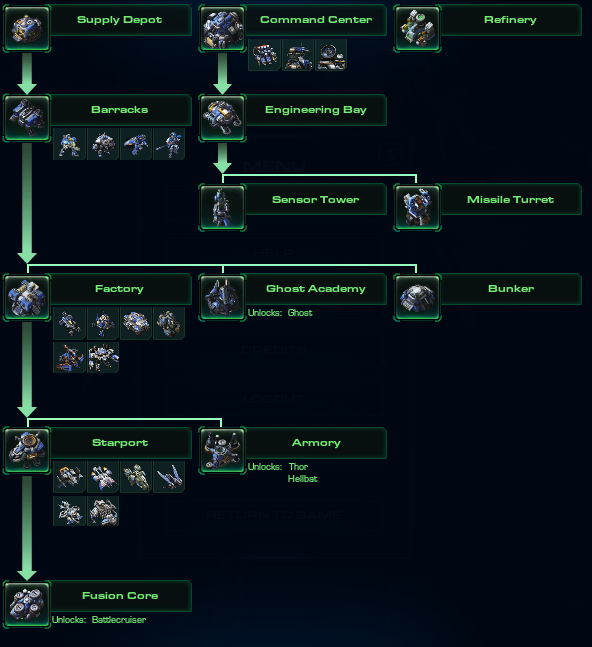
\includegraphics[keepaspectratio]{images/2.png}
	\captionimg{Árbol de tecnologías}{(Blizzard Entertainment, 2021)}
	\label{fig:2}
\end{figure}

\subsection{Economía}

Cómo todo en la vida, cualquiera de las fuerzas previamente mencionadas viene con un costo que varía según la utilidad de cada una. Existen dos tipos de \textbf{recursos} no renovables (minerales y gas vespeno), representados en el juego por números enteros, que son obtenidos por medio de los trabajadores y que son sustraídos cada vez que la creación de una entidad lo requiera y en las cantidades que se especifique. Es importante aclarar que estos recursos no pueden ser menores que cero en ningún caso.

Los \textbf{minerales} son la fuente principal de recursos en StarCraft II, pues todas las entidades lo requieren para comenzar su proceso de creación. Estos minerales son extraídos directamente de los campos de minerales que se encuentran en el mapa por los \textit{SCV}, para luego ser llevados a un \textit{Command Center} (o cualquier edificio que evolucione de este) en donde pasan a ser contabilizados en la cantidad de minerales obtenidos.

\begin{figure}[H]
	\centering
	\captionsetup{justification=centering}
	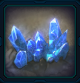
\includegraphics[keepaspectratio]{images/minerals.png}
	\captionimg{Minerales}{(Blizzard Entertainment, 2021)}
	\label{fig:3}
\end{figure}

Al comienzo de la partida, la base del jugador inicia en la cercanía de cuatro campos de minerales grandes (que otorgan un máximo de 1800 minerales cada uno) y cuatro pequeños (900 minerales cada uno) resultando en un máximo total de 10800 minerales por base. Si bien estos recursos son limitados y no renovables, el jugador puede encontrar nuevos campos de minerales a lo largo del mapa en las mismas cantidades que los que aparecen en la base inicial, para los cuales es recomendable construir un nuevo \textit{Command Center} que permita depositar el mineral de forma más expedita.

A la hora de extraer los minerales, un \textit{SCV} tarda 1.99 segundos desde que comienza hasta que obtiene los 5 de mineral que puede cargar para, luego, esperar por, aproximadamente, 0.3571 segundos antes de devolverse al \textit{Command Center} para depositarlos y generar un \textbf{ingreso} de 5 minerales. Debido a que sólo se admite un trabajador por mineral a la vez, es que ocurre un fenómeno denominado \textbf{saturación} en dónde se busca maximizar el ingreso al minimizar la aparición de colas de trabajadores que intentan acceder a un mismo mineral, pues cada segundo a la espera es un segundo perdido. Básicamente, hasta dos \textit{SCV} pueden encargarse de un mismo mineral sin que tengan que esperar a que el otro finalice (ambos tienen una \textbf{eficiencia} del 100\% en cuanto al ingreso que obtienen), pero, al ser el objetivo principal el de recolectar la mayor cantidad posible de mineral en el tiempo, es que se ha calculado que el óptimo es de 3 trabajadores por mineral (demostrado visualmente en el juego con un total de 24 \textit{SCV} por base), donde el tercer trabajador recibe menos minerales por unidad de tiempo, pero se maximiza el ingreso total por cada mineral. Con esto en mente, los cálculos realizados por un usuario de la comunidad de StarCraft II (PiousFlea, 2010) arrojan un total aproximado de 102 minerales por minuto al contar con 3 trabajadores por mineral.

Un caso particular ocurre con la unidad \textit{MULE} que puede obtener 4 veces los minerales que un \textit{SCV} y no satura los minerales (ignora las colas), pero con la diferencia de que es una unidad temporal que desaparece pasados 65 segundos desde su creación, cuyo único requisito es la utilización de energía desde un \textit{Orbital Command}. La \textbf{energía} es un recurso renovable que es característico sólo a algunas entidades como el \textit{Orbital Command}, pero que sólo es utilizado para la creación instantánea de otras entidades por este último en la creación de un \textit{MULE} o la investigación de \textit{Extra Supplies}, mientras que el resto de las entidades que poseen energía, la gastan en el uso de distintas habilidades. Las entidades suelen comenzar con 50 de energía, la cual aumenta en 0.7875 cada segundo hasta un máximo de 200, siendo este recurso independiente para cada instancia de entidad.

Por otro lado, el \textbf{gas vespeno} es un recurso más limitado (sólo dos \textbf{géiseres} de gas por base) que no necesitan todas las unidades, pero que no deja de ser vital para construir entidades más poderosas que las que requieren solamente del mineral. A diferencia del anterior que puede ser extraído directamente de los géiseres de gas, el gas vespeno necesita de la creación de un \textit{Refinery} para que los \textit{SCV} puedan extraer el recurso y llevarlo al \textit{Command Center} para que se agregue a la cantidad de gas total.

\begin{figure}[H]
	\centering
	\captionsetup{justification=centering}
	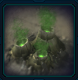
\includegraphics[keepaspectratio]{images/gas.png}
	\captionimg{Géiseres de gas vespeno}{(Blizzard Entertainment, 2021)}
	\label{fig:4}
\end{figure}

Para la extracción de gas, un \textit{SCV} tarda 1.415 segundos en la extracción del recurso desde el \textit{Refinery} y se dirige inmediatamente a la base a depositar un ingreso igual a los 4 de gas vespeno. Al igual que los minerales, el gas vespeno alcanza la saturación a los 3 trabajadores (total de 6 por base), dando un total de 114 de gas por minuto.

Catalogado también como recurso, aunque con un comportamiento muy distinto al de los dos anteriormente vistos, se tiene el suministro, que es un requisito exclusivo de las unidades. El \textbf{suministro} es un valor entero que limita la cantidad de unidades que se pueden poseer, pues cada una tiene un valor definido que va desde 1 hasta 6 y que se suma para obtener la cantidad actual de suministro del ejército de cada jugador y que debe ser menor que el \textbf{suministro total} que ofrecen algunos edificios. El suministro total es simplemente la suma de 15 veces la cantidad de \textit{Command Centers} o edificios que evolucionen de este más 8 veces la cantidad de \textit{Supply Depots} (edificio) o 16 veces si es que el \textit{Supply Depot} tiene un \textit{Extra Supplies} vinculado. En el caso de agregar una unidad a la cola de creación de cualquier edificio y que el valor de los suministros actuales (contando a la unidad que se desea construir) exceda el de los suministros totales, esta unidad no podrá ser puesta en cola hasta que los suministros totales aumenten.

\subsection{Velocidad de juego}

Al tratarse de un juego en tiempo real es normal que las acciones sean medidas en segundos o fracciones de estos, pero dado que StarCraft II introduce la función de cambiar la \textbf{velocidad de juego} es que se debe explicar en que consiste para poner todo bajo el mismo contexto. El videojuego ofrece cinco velocidades de juego que pueden ser escogidas al crear una partida personalizada o es establecida en la velocidad más alta en caso de que se trate de una partida con emparejamiento automático (partidas clasificatorias). Los \textbf{factores de velocidad} de cada velocidad de juego, cuyos valores están indicados en la tabla {\ref{tab:1}}, dividen los segundos reales para calcular el tiempo de los elementos del juego que lo requieran.

\begin{table}[H]
\centering
\def\arraystretch{1.8}
\captionsetup{justification=centering}
\caption{Tabla de velocidades de juego}
\label{tab:1}
\resizebox{\textwidth}{!}{%
\begin{tabular}{|c|c|c|}
\hline
\textbf{Velocidad de Juego} & \textbf{Factor de Velocidad} & \textbf{Segundos de Tiempo Real en 1 Minuto de Juego \textit{Normal}} \\
\hline
Slower & 0.6 & 100 \\ \hline
Slow & 0.8 & 75 \\ \hline
Normal & 1.0 & 60 \\ \hline
Fast & 1.2 & 50 \\ \hline
Faster & 1.4 & 42.86 \\ \hline
\end{tabular}%
}
\caption*{\textbf{Fuente}: Elaboración Propia, 2021}
\end{table}

Para ejemplificar lo anterior, se puede decir que un \textit{Supply Depot}, que tarda 30 segundos reales en crearse a una velocidad de juego \textit{normal}, tardará aproximadamente 21 segundos reales (21.423, pero el juego aproxima estos valores a un número entero) al utilizar la velocidad de juego \textit{faster}.

La lectura de este documento debe ser abordada teniendo en cuenta la velocidad de juego \textit{faster} como la velocidad por defecto, que es la que se utiliza en partidas clasificatorias y en torneos oficiales. Con esto presente, es importante aclarar que los valores en tiempo mencionados en las secciones anteriores, así como en las secciones por venir, son los que se obtienen en el juego al usar esta velocidad de juego \textit{faster}, lo cual afecta principalmente a los tiempos que tardan en crearse las entidades y los tiempos en que los trabajadores recolectan recursos.

\subsection{Órdenes de construcción}

Si bien ya han sido mencionados a lo largo del documento, aún no se establece una definición concreta sobre los órdenes de construcción.

Cada vez que un jugador comienza la producción de una unidad, la construcción de un edificio o la investigación de una mejora se dice que el jugador está realizando una \textbf{acción}, la cual ocurre en un tiempo determinado contado a partir del inicio de la partida. Al reunir estas acciones en una secuencia, ordenada según sus marcas de tiempo respectivas, se tiene lo que se denomina \textbf{orden de construcción} (conocido en inglés como \textit{Build Order}), el cual se muestra al final de cada partida. Este término no es usado sólamente para referirse a las secuencias que aparecen después de una partida, sino que también se habla de estas series de acciones para referirse a órdenes de construcción "ideales", los cuales tienen las mismas características, pero son secuencias ideales que un jugador debe seguir para alcanzar una o varias entidades deseadas.

Es habitual en la comunidad de StarCraft II que los jugadores compartan estos órdenes de construcción con la finalidad de que sean evaluados por otros jugadores, por lo que no es extraño que se observen distintos formatos a la hora de presentarlos, algunos con elementos extra que facilitan la visualización y comprensión de los mismos. A modo de ejemplo de esto, se puede observar en la figura {\ref{fig:1}} como un orden de construcción puede tener otros valores además de los dos principales (el tiempo y la entidad construida) como la cantidad de suministros máximos y la cantidad de suministros actuales para entregar mayor contexto de la partida, así cómo también existen formatos que utilizan esto último para no incluir la creación de trabajadores con el fin de acortar el tamaño total del orden de construcción.

\begin{figure}[H]
	\centering
	\captionsetup{justification=centering}
	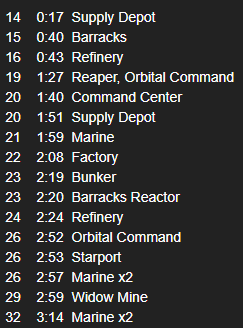
\includegraphics[keepaspectratio]{images/1.png}
	\captionimg{Parte de un orden de construcción}{(Spawning Tool, 2021)}
	\label{fig:1}
\end{figure}

\section{StarCraft II como problema de optimización}

El \textbf{problema de planificación de proyecto con recursos limitados} (Artigues, 2008), mejor conocido como RCPSP (\textit{Resource Constrained Project Scheduling Problem}), es un problema de optimización combinatorial que involucra el manejo de los distintos requisitos obligatorios asociados a un problema con el fin de obtener una \textbf{planificación} de duración mínima, siempre respetando las relaciones de precedencia existentes y la disponibilidad de los recursos.

Un RCPSP se considera como tal al poseer \textbf{actividades} que componen el problema, cuyo inicio se representa como una marca de tiempo denominada \textit{\textbf{schedule}}, y que pueden ser vistas como hitos dentro de esta, además de que cada una de estas actividades tiene una \textbf{duración} asignada y \textbf{relaciones de precedencia} que obligan a que una actividad $A_{j}$ necesite de una previa actividad $A_{i}$ antes de comenzar. Estas actividades no solo requieren de otras, sino que, también, se ven afectadas por la \textbf{demanda} de \textbf{recursos renovables} con distinta \textbf{disponibilidad}.

Con esto en mente y luego de contrastar el RCPSP con las características del videojuego, quedan en evidencia las similitudes entre ambos problemas, permitiendo declarar el \textit{problema de los órdenes de construcción} como un problema de planificación de proyecto con recursos limitados. Las \textit{actividades} describen a la perfección a la creación de las distintas entidades que componen un orden de construcción, pues cada una de ellas tiene una \textit{duración} particular desde que inicia su creación y \textit{relaciones de precedencia} en las distintas entidades requisito que cada una posee. Y esto no es todo, pues la creación de entidades también \textit{demanda} suministros, además de los \textit{recursos renovables}, mineral y gas vespeno cuyas \textit{disponibilidades} varían según la cantidad de trabajadores y su ubicación en el mapa. Para ejemplificar esto, se usa a la unidad \textit{Ghost}, cuya creación tarda 29 segundos en un tiempo de juego \textit{faster}, que debe ser construida en el edificio \textit{Barracks}, pero también requiere que el edificio \textit{Ghost Academy} haya sido creado antes de poder iniciar su propia creación, la cual necesita 150 de mineral, 125 de gas vespeno y al menos 2 de suministro disponible.

\section{Metaheurísticas}

Aún sin garantía de encontrar el óptimo global, las metaheurísticas permiten atacar problemas de optimización para obtener soluciones satisfactorias en un tiempo razonable (Young, 2009). La palabra \textbf{heurística} viene del griego \textit{heuriskein} que se refiere al "arte de descubrir nuevas estrategias o reglas para resolver problemas", mientras que el \textit{meta} en metaheurística significa "metodología de nivel superior", por lo que las \textbf{metaheurísticas} se definen como metodologías generales de nivel superior que pueden ser usadas como estrategias guía al diseñar heurísticas adyacentes para resolver problemas de optimización específicos.

Existen diversos métodos para clasificar a las metaheurísticas. Un ejemplo de esto es clasificarlas según su inspiración al separar aquellas metaheurísticas inspiradas en la naturaleza de las no inspiradas en la naturaleza, pero en esta oportunidad usará la clasificación según el tipo de solución sobre la que trabaja el algoritmo: algoritmos basados en población y algoritmos basados en solución única.

\subsection{Algoritmos de población}

Los \textbf{algoritmos de población} son un tipo de metaheurísticas, los cuales pueden ser vistos como una evolución de una población (conjunto) de soluciones que, de forma iterativa, se va integrando con la población de soluciones actual por medio del uso de procedimientos de selección, permitiendo una mejor diversificación en el espacio de búsqueda, de forma complementaria a los algoritmos de solución única. Ejemplos de este tipo de metaheurística se pueden ver en \textit{algoritmos evolucionarios}, \textit{scatter search} y \textit{algoritmos de estimación de distribución}.

\subsection{Algoritmos de solución única}

Aquellas metaheurísticas que, a diferencia de los algoritmos de población, buscan mejorar sólo una solución son denominadas como \textbf{algoritmos de solución única}, pues recorren el espacio de búsqueda saltando de una solución actual a otra de forma iterativa con la intención de acercarse al óptimo global al intensificar la búsqueda en regiones locales. Algunos ejemplos de este tipo de metaheurísticas son \textit{Simulated Annealing}, \textit{Local Search} y \textit{Tabu Search}.

Entre los conceptos comunes para las metaheurísticas con algoritmos de solución única se encuentran los \textbf{vecindarios}, estructuras de soluciones asociadas a una solución particular, o las \textbf{soluciones iniciales}, que son utilizadas para comenzar cada algoritmo y que puede ser obtenida de manera aleatoria o con un acercamiento \textit{greedy}.

\subsection{Simulated Annealing}

La solución propuesta consta del modelo bajo un enfoque metaheurístico, que incluye un algoritmo capaz de encontrar buenos órdenes de construcción para llegar a una unidad, una tecnología o una estructura de la raza Terran en StarCraft II. Esto, según se especifique antes de la ejecución del algoritmo y optimizando el criterio del tiempo de partida para llegar a dicha unidad, estructura o tecnología. La metaheurística a utilizar será \textbf{\textit{Simulated Annealing}} (SA a partir de ahora), la cual es una metaheurística de algoritmo de solución única que busca imitar el proceso de recocido de algunos metales para obtener el material en un estado más puro o, en este caso, acercarse al óptimo. Si se ve como algoritmo, SA tiene como objetivo escapar del óptimo local de forma en que las generaciones no queden atrapadas en una solución particular. Comenzando con una solución inicial, SA genera un vecino en cada iteración, el cual es seleccionado siempre que mejore la función de costo, pero que en caso de que no mejore esta función, tiene una probabilidad de ser seleccionado según la temperatura (parámetro de control definido acorde al problema) y la diferencia entre los resultados de la función objetivo de las soluciones en comparación. \newline

\begin{algorithm}[H]
    \SetKwData{Left}{left}
    \SetKwData{This}{this}
    \SetKwData{Up}{up}
    \SetKwFunction{Union}{Union}
    \SetKwFunction{FindCompress}{FindCompress}
    \SetKwInOut{Input}{input}
    \SetKwInOut{Output}{output}

    \KwIn{Calendario de enfriamiento}
    \caption{Simulated Annealing}\label{alg:sa}
    
    $s \gets s_{0}$; \tcc{Generación de la solución inicial}\
    $T \gets T_{0}$; \tcc{Temperatura inicial}
    
    \While{Criterio de detención no satisfecho}{
        \While{Condición de equilibrio no satisfecha}{
            Se genera un vecino aleatorio $s'$\;
            $\Delta E \gets f(s') - f(s)$\;
            \If{$\Delta E \leq 0$}{
                $s \gets s'$; \tcc{Acepta la solución vecina}
            }
            \Else{
                $s \gets s'$;\tcc{Acepta s' con una probabilidad $e^\frac{-\Delta E}{T}$}
            }
        }
        $T \gets g(T);$ \tcc{Actualización de temperatura}
    }
    \KwOut{Mejor solución encontrada} 
\end{algorithm}

\section{I-Race}

Aún antes de ejecutar el algoritmo para optimizar las soluciones, es importante optimizar los parámetros que SA recibe con la finalidad de obtener los mejores resultados posibles; a este proceso recién descrito se le denomina \textbf{parametrización}. Ahora, utilizando el paquete de R \textit{\textbf{i-race}} es posible conseguir esta parametrización de forma automática al entregarle conjuntos o rangos de posibles parámetros para que el algoritmo de \textit{i-race} ejecute reiteradamente el algoritmo cuyos parámetros se busca optimizar, que en este caso se trata de SA aplicado al problema de los órdenes de construcción, hasta que se cumpla el \textbf{presupuesto} o número de ejecuciones previamente ajustado. Finalmente se obtendrá una tabla con los mejores parámetros posibles de entre los entregados, el cual debe ser utilizado en las futuras ejecuciones del algoritmo SA.




\chapter{Algoritmo propuesto y experimentos}

En este capítulo se detalla el algoritmo incluido en el modelo propuesto, además de los experimentos a realizar para probar la aplicación de este algoritmo.

\section{Algoritmo propuesto}

Con la finalidad de cumplir con lo estipulado en el objetivo principal, se requiere una explicación de los pasos, los cuales son detallados en este capítulo para darle forma a la solución computacional que apunta a resolver el problema.

El algoritmo \textit{Simulated Annealing} tiene 3 parámetros de entrada que son necesarios para su ejecución, los cuales son la \textbf{temperatura} inicial, \textit{T}, el \textbf{calendario de enfriamiento}, dado por \(T * \)$\alpha$, y la \textbf{generación inicial}, $G_{0}$. Esto, sin contar con las entradas principal del modelo, los cuales son la \textbf{entidad objetivo}, $E$, para la que se requiere obtener un orden de construcción y la \textbf{cantidad} $Q_{E}$ de la entidad objetivo que se desee. Además se opta por que los \textbf{ciclos} estén establecidos desde un inicio en los parámetros \textit{N} para las iteraciones externas y \textit{M} para los ciclos internos.

La generación inicial es aleatoria y con una duración en tiempo de juego, \textit{t}, también aleatoria, pero con un tiempo de juego máximo definido previamente como un \textbf{intervalo}, \textit{I}, que se aplica en cada generación. La cantidad $Q_{E}$ debe ser un entero igual o mayor a 1. Por otro lado, la temperatura $T$ es un entero al inicio, pero a lo largo del algoritmo puede tomar valores decimales al ser multiplicado por $\alpha$ que es un decimal entre 0 y 1 sin incluir a este último. \newline

\begin{algorithm}[H]
    \SetKwData{Left}{left}
    \SetKwData{This}{this}
    \SetKwData{Up}{up}
    \SetKwFunction{Union}{Union}
    \SetKwFunction{FindCompress}{FindCompress}
    \SetKwInOut{Input}{input}
    \SetKwInOut{Output}{output}

    \KwIn{$T, \alpha, G_{0}, N, M, I, E, Q_{E}$}
    \KwOut{Generación $G_{Best}$ del orden de construcción}    
    \caption{Simulated Annealing aplicado al problema de los órdenes de construcción}\label{alg:sa4bo}
    
    \tcc{Inicialización de generación}
    $P, P_{Best} \gets puntaje(G_{0})$\;
    $G_{SA}, G_{Best} \gets G_{0}$\;
    
    \For{\textit{n en N}}{
        \For{\textit{m en M}}{
            \tcc{Corte aleatorio de la generación actual}
            $t_{o} \gets entero\_aleatorio(0, t_{G_{SA}})$\;
            $G \gets recrear\_generacion(G_{SA}, t_{o})$\;
            \tcc{Generación aleatoria a partir de la generación actual}
            $t_{f} \gets t_{o} + entero\_aleatorio(0, I)$\;
            $G' \gets oc\_aleatorio(G, t_{o}, t_{f}, E, Q_{E})$\;
            \tcc{Cálculo del puntaje y diferencia entre estos}
            $P' \gets puntaje(G')$\;
            $\Delta_{P} \gets P' - P$\;
            \tcc{Comparación con la generación actual}
            \If{$\Delta P < 0$}{
                $G_{SA}, P \gets G', P'$\;
            }
            \Else{
                $prob \gets exp(\Delta_{P}/T)$\;
                $prob\_acep \gets decimal\_aleatorio(0, 1)$\;
                \If{$prob\_acep < prob$}{
                    $G_{SA}, P \gets G', P'$\;
                }
            }
            \tcc{Comparación con la mejor generación}
            \If{$P' < P_{Best}$}{
                $G_{Best}, P_{Best} \gets G', P'$\;
            }
        }
        $T \gets T * \alpha$\;
    }
\end{algorithm}



\subsection{Representación de los datos}

Si bien el algoritmo ya está diseñado, es necesario tomar los elementos del videojuego que se incluyen en la solución e implementarlos para poder implementar \textit{Simulated Annealing}. Un caso importante de esto, es que las entidades tienen asignado un número entero para cada una, el cual es utilizado en gran parte de las representación a continuación.

Lo más importante a representar son las \textbf{generaciones}, ya que son equivalentes a las soluciones que entregue el algoritmo. Las cuales fueron divididas en cinco tablas con toda la información necesaria y se explican en las secciones a continuación.

\subsubsection{Acciones}

La tabla de \textbf{acciones} que es, básicamente, el orden de construcción ya que guarda la entidad a construir y la marca de tiempo (en velocidad \textit{faster}) de cada entidad que se crea. Esto en cada fila la tabla.

\begin{table}[H]
\centering
\def\arraystretch{1.8}
\captionsetup{justification=centering}
\caption{Tabla de acciones}
\label{tab:4}
\begin{tabular}{|c|c|}
\hline
\textbf{Entidad} & \textbf{Marca de Tiempo} \\
\hline
SCV & 2 \\ \hline
Refinery & 10 \\ \hline
SCV & 17 \\ \hline
Supply Depot & 32 \\ \hline
Refinery & 42 \\ \hline
\end{tabular}
\caption*{\textbf{Fuente}: Elaboración Propia, 2021}
\end{table}

\subsubsection{Edificios}

Se tiene también una tabla para los \textbf{edificios} que indica el estado de estos en un segundo particular de la solución, la cual almacena los edificios creados y tiene \textbf{espacios de creación} disponibles para cada edificio (con la posibilidad de un segundo espacio para los edificios con un \textit{Reactor} que pueden construir dos unidades a la vez) con su \textbf{utilización} asociada para medir el tiempo (representado por un entero) restante en la creación de cada unidad, la cual se actualiza en cada segundo de la solución; el último valor es el de la \textbf{energía}, que nos muestra la energía actual del edificio en cuestión y es un número flotante.

Para los espacios de creación existe un valor 0 que representa cuando dicho espacio no está siendo utilizado y -1 en caso de que el espacio no esté habilitado. La utilización se reduce en 1 por cada segundo real, excepto cuando es 0, pues significa que la entidad ya fue construida o simplemente no existe una en creación. Finalmente, la energía es un flotante con un tope de 200 y que aumenta 0.7875 por segundo, pero que sólo se cuenta para el \textit{Orbital Command}.

\begin{table}[H]
\centering
\def\arraystretch{1.8}
\captionsetup{justification=centering}
\caption{Tabla de edificios}
\label{tab:5}
\begin{tabular}{|c|c|c|c|c|c|}
\hline
\textbf{Edificio} & \textbf{Espacio 1} & \textbf{Utilización 1} & \textbf{Espacio 2} & \textbf{Utilización 2} & \textbf{Energía} \\
\hline
Supply Depot & Sin utilizar & 0 & No aplica & 0 & 0 \\ \hline
Refinery & Sin utilizar & 0 & No aplica & 0 & 0 \\ \hline
Refinery & Sin utilizar & 0 & No aplica & 0 & 0 \\ \hline
Command Center & Sin utilizar & 0 & No aplica & 0 & 0 \\ \hline
Barracks & Marine & 17 & No aplica & 0 & 0 \\ \hline
\end{tabular}
\caption*{\textbf{Fuente}: Elaboración Propia, 2021}
\end{table}

\subsubsection{Trabajadores}

Con un acercamiento similar a los edificios, la tabla de \textbf{trabajadores} muestra el estado de los \textit{SCV} y los \textit{MULE} en un segundo particular. Existe una columna para los \textbf{espacios de creación} que funciona de igual manera que en los edificios, además de la utilización para cada edificio que se esté creando. Lo que separa esta tabla de la anterior, es que no existe la energía, ni una segunda columna para otro espacio de creación o su utilización asociada, pero en su lugar existe una \textbf{duración} que indica el tiempo restante (como entero) que le queda al \textit{MULE} antes de desaparecer.

A diferencia de los edificios, los espacios de creación pueden tomar un valor mayor que 0, igual al edificio que representan; 0 en caso de que que el trabajador no esté siendo utilizado; -1 en caso de que se encuentre extrayendo minerales; o -2 en caso de que se encuentre recolectando gas vespeno.

\begin{table}[H]
\centering
\def\arraystretch{1.8}
\captionsetup{justification=centering}
\caption{Tabla de trabajadores}
\label{tab:6}
\begin{tabular}{|c|c|c|c|}
\hline
\textbf{Trabajador} & \textbf{Espacio} & \textbf{Utilización} & \textbf{Duración} \\
\hline
SCV & Gas & 0 & No aplica \\ \hline
SCV & Gas & 0 & No aplica \\ \hline
SCV & Gas & 0 & No aplica \\ \hline
SCV & Supply Depot & 5 & No aplica \\ \hline
SCV & Minerales & 0 & No aplica \\ \hline
SCV & Minerales & 0 & No aplica \\ \hline
\end{tabular}
\caption*{\textbf{Fuente}: Elaboración Propia, 2021}
\end{table}

\subsubsection{Entidades}

Esta tabla indica las \textbf{entidades} que existen en un punto determinado de cada generación al tener una columna con cada \textbf{entidad} de la raza Terran, además de una columna con la \textbf{cantidad} de cada una de estas. El fin de esta tabla es la de reducir tiempo de procesamiento al no tener que contar las entidades cada vez que se necesite saber la cantidad de alguna de estas.

\begin{table}[H]
\centering
\def\arraystretch{1.8}
\captionsetup{justification=centering}
\caption{Fragmento de la tabla de entidades}
\label{tab:7}
\begin{tabular}{|c|c|}
\hline
\textbf{Identificador de entidad} & \textbf{Cantidad} \\
\hline
1 & 1 \\ \hline
2 & 1 \\ \hline
3 & 2 \\ \hline
4 & 1 \\ \hline
5 & 1 \\ \hline
14 & 0 \\ \hline
17 & 1 \\ \hline
18 & 0 \\ \hline
19 & 0 \\ \hline
20 & 0 \\ \hline
21 & 18 \\ \hline
\end{tabular}
\caption*{\textbf{Fuente}: Elaboración Propia, 2021}
\end{table}

\subsubsection{Recursos}

Una tabla que muestra los \textbf{recursos} en cada segundo de la solución. Cada fila posee el \textbf{tiempo} que avanza de 1 en 1, la cantidad flotante de \textbf{minerales}, la cantidad flotante de \textbf{gas vespeno} y la cantidad de\textbf{suministros máximos} como un entero.

Aunque los minerales y gas vespeno en el juego sólo toman valores enteros, se utilizan decimales debido al aproximado de recolección por segundo. Para el tiempo, se utiliza 0 como el valor al comenzar la partida y mayor que 0 para todos los segundos que le siguen.

\begin{table}[H]
\centering
\def\arraystretch{1.8}
\captionsetup{justification=centering}
\caption{Tabla de recursos}
\label{tab:8}
\begin{tabular}{|c|c|c|c|}
\hline
\textbf{Tiempo (en segundos)} & \textbf{Minerales} & \textbf{Gas Vespeno} & \textbf{Suministros} \\
\hline 
0 & 50.000 & 0.000 & 0 \\ \hline
1 & 57.500 & 0.000 & 15 \\ \hline
2 & 65.000 & 0.000 & 15 \\ \hline
3 & 22.500 & 0.000 & 15 \\ \hline
4 & 30.000 & 0.000 & 15 \\ \hline
5 & 37.500 & 0.000 & 15 \\ \hline
\end{tabular}
\caption*{\textbf{Fuente}: Elaboración Propia, 2021}
\end{table}

\subsubsection{Árbol de tecnologías}

El árbol de tecnologías se ve representado en una tabla cuyas filas representan el \textbf{identificador} de cada entidad, las cuales incluyen el \textbf{nombre} de cada entidad a fin de presentarlas cuando corresponda, el \textbf{tiempo de construcción} como un entero, la \textbf{entidad de construcción} como un entero correspondiente a la fila de la entidad, la cantidad (como entero) de los distintos \textbf{recursos} que cada entidad necesita para construirse, además de los requisitos como si requieren una entidad previa que les \textbf{desbloquee}, si es que es una \textbf{mejora} de otra mejora ya existe o si es un edificio que \textbf{evolucione} de otro. Esta tabla se encarga de proveer la información particular de cada unidad, tecnología y mejora para los distintos operadores de la solución, volviéndose una tabla de lectura a diferencia de las tablas que componen las generaciones.

A excepción del nombre, todos los datos toman valores enteros, siendo 0 el mínimo y -1 en caso de que dicha variable no aplique para alguna entidad (por ejemplo, un \textit{Marine} no tiene es desbloqueado por otra entidad ni se transforma desde alguna entidad particular). Como ya se explicaba, el identificador de cada entidad está dado por el número de fila al que corresponda, iniciando con un edificio que no existe en el juego (\textit{Townhall} en la posición 1) a modo de tener el grafo, formado por este árbol de tecnologías, unido en un mismo nodo inicial.

\subsection{Criterios de optimización}

Existen diversos criterios que pueden ser optimizados en un orden de construcción, siendo el \textit{tiempo de juego} para la entidad a la que se desea llegar el criterio que se busca optimizar en esta ocasión, dejando a un lado criterios como la cantidad de entidades totales obtenidas, que es inversamente proporcional al tiempo de juego debido a que más entidades requerirán una mayor cantidad de tiempo, o la fuerza del ejército formado, lo cuál requiere algo más de trabajo pues esta \textit{fuerza} no es un valor que el juego entregue ni que se pueda deducir objetivamente o con facilidad.

\subsection{Operadores}

La solución posee distintos operadores que apoyan al algoritmo \textit{Simulated Annealing}, que se puede ver en pseudo-código en el algoritmo \ref{alg:sa4bo}, los cuales son detallados en las secciones a continuación.

\subsubsection{Orden de construcción aleatorio}

Una de las funciones principales (utilizada en la línea 8 del algoritmo \ref{alg:sa4bo}) que permite la creación de una generación al entregarnos todas las tablas que las componen. Recibe las tablas de una generación, que pueden ser las iniciales en caso de que sea la primera generación, el tiempo de inicio de la nueva generación (denotado por el tiempo final de la generación que se le entrega) para comenzar a armar la solución 1 segundo después del indicado y el tiempo de fin que indica el tamaño (en tiempo) de la solución.

Este algoritmo consiste en actualizar todas las tablas cada segundo desde el de inicial + 1 hasta el tiempo de fin. Cada ciclo incluye la elección al azar de una de las posibles entidades a crear (que sólo se crea si cumple todos sus requisitos) y la actualización de las tablas de la generación al reducir los segundos de las entidades a la espera de ser creadas y agregar cualquiera que fuera creada durante el ciclo en los lugares correspondientes.

Finalmente, el algoritmo entrega las tablas de la generación obtenida.

\subsubsection{Puntaje}

Es el operador que se encarga de entregar el puntaje de una solución en concreto (utilizado en las líneas 1 y 9 del algoritmo \ref{alg:sa4bo}) o, en otras palabras, es la función objetivo que se utiliza en \textit{Simulated Annealing} para comparar las generaciones dentro de los ciclos.

El cálculo del puntaje se realiza en cada generación del algoritmo para chequear si la nueva solución \(G'\) es mejor o peor que la solución actual $G_{SA}$ o la mejor solución $G_{Best}$ y posee dos componentes principales: el puntaje de las entidades y el puntaje del tiempo.

El puntaje de las entidades se calcula según la entidad objetivo $E$ y la cantidad de la entidad objetivo $Q_{E}$ que se indiquen al operador. En esencia, el puntaje de las entidades mide cuántas entidades faltan para llegar a la entidad objetivo al usar la cantidad de entidades requisitos $Q_{R}$ de la entidad objetivo $E$ (con los requisitos de los requisitos siendo parte de este total) junto a la cantidad de la entidad $Q_{E}$ para obtener el total necesario \(Q_R + Q_{E}\). Con la finalidad de normalizar este valor para que su resultado sea entre 0 y 1 es que queda \(P_{E} = \frac{Q_R_i + Q_E_i}{Q_R + Q_E}\), con $Q_{R}_i$ y $Q_{E}_i$ como la diferencia entre las entidades actuales en el orden de construcción y las entidades totales requeridas.

De forma más simple, el puntaje del tiempo $P_t$ originalmente se pensó normalizar para que el valor estuviera entre 0 y 1 y luego ponderarlo con el puntaje de las entidades, pero dadas las características de SA, en dónde se compara una solución directamente con otra, es que este acercamiento sólo permitía la comparación a nivel localizado entre una solución $G$ y su vecino $G'$, pero al utilizar el máximo y mínimo de todos los tiempos obtenidos en la ejecución del algoritmo es que, al graficar estos datos, el puntaje de la solución $G_{Best}$ que, en teoría, sólo debe disminuir presentaba aumentos. Ante esto, se optó por ponderar sólo $P_E$ y utilizar el tiempo de juego en bruto como $P_t$.

Con lo anterior, una vez calculados ambos puntajes $P_t$ y $P_E$ es que el puntaje de las entidades $P_E$ pasa por una función $f(P_E) = P_E * I * (Q_R + Q_E + 1)$, siendo $I$ el intervalo de tiempo máximo, con el fin de darle mayor importancia a las entidades necesarias para alcanzar la entidad objetivo que al tiempo de juego total de la solución, intentando que la diferencia de estos tiempos sea menor al puntaje ponderado de un orden de construcción con una entidad más cerca de llegar al objetivo. Finalmente se consigue una ponderación $P = P_t + f(P_E) $

\subsubsection{Recrear generación}

Operador encargado de recrear las tablas de las generaciones en un segundo de tiempo de juego en concreto (utilizado en la líneas 6 del algoritmo \ref{alg:sa4bo}), el cual recibe el segundo en que se desea recrear la generación (debe ser menor que el máximo) y las tablas de la generación.

Este operador inicia cortando la tablas de recursos en el tiempo indicado y la tabla de acciones para que incluya las acciones que ocurren durante o previas al segundo especificado. La siguiente es la tabla de entidades que puede recrearse a partir de la tabla de acciones. Ya con estas tablas, sólo resta volver a armar las tablas de trabajadores y edificios al llenarlas con la tabla de entidades y poblar sus espacios con la ayuda de la tabla de acciones.

\subsection{Ciclo del algoritmo}

Teniendo en cuenta los operadores anteriores y el algoritmo \ref{alg:sa4bo}, se distingue la existencia de dos ciclos, uno externo y otro interno, con N y M iteraciones respectivamente.

El ciclo interno (desde la línea 4 a la 24) inicia creando una solución $G'$ vecina a partir de orden de construcción $G_{SA}$ cortado en un tiempo de juego aleatorio $t_o$ dentro de su duración con un largo igual a $t_o + t_f$, con $t_f$ un tiempo de juego aleatorio entre 0 y el intervalo máximo $I$. Luego se calcula el puntaje $P'$ de dicha solución y la diferencia $\Delta P$ de este con el puntaje actual $P$ con la cual se calcula la probabilidad de aceptar la solución con puntaje $P'$ en caso de que este sea mayor al de $P$, pues una solución menor siempre se acepta. Luego se reemplaza en el caso de que la solución $G'$ tenga un mejor puntaje que $G_{Best}$.

El ciclo externo se compone por el ciclo interno y la línea 25 en dónde la temperatura se actualiza según el calendario de enfriamiento dado por $\alpha$, lo cual ocasiona que la probabilidad de aceptación en caso en que $\Delta P$ sea menor tras cada iteración externa.

\section{Diseño experimental}

Para conseguir los objetivos propuestos es necesario realizar diversos experimentos cuyos resultados permitan llegar a una conclusión respecto al algoritmo SA y su implementación con el problema de los órdenes de construcción, por lo que a continuación se detallan los diversos experimentos llevados a cabo en este documento.

\subsection{Parametrización}

Utilizando el paquete de R \textit{i-race} para la parametrización, se le entregan los rangos de los ciclos internos, la temperatura, $\alpha$ usado para el enfriamiento y el intervalo máximo. Se tiene que para el ciclo interno los valores enteros van entre las 25 y 250 iteraciones, el rango de la temperatura oscila entre 500 y 50000, $\alpha$ puede ser un valor entre 0.5 y 0.99 y, finalmente, un intervalo máximo entre 30 y 180 segundos considerando el tiempo de juego \textit{faster}. De estos valores, los que más influyen en el tiempo de ejecución son el ciclo interno y el intervalo máximo. Aunque el ciclo externo también es un valor importante a optimizar, se deja como 50 tanto para la parametrización cómo para la ejecución del algoritmo, pues el tiempo necesario para obtener una solución se eleva demasiado al aumentar este número según lo observado en una etapa previa de pruebas del funcionamiento del algoritmo.

Para el presupuesto de la parametrización se utiliza un valor de 180, el cual define también la cantidad de ejecuciones que realizará \textit{i-race} antes de entregar su respuesta.

\subsection{Evaluación}

Para poder llegar a una conclusión respecto a la hipótesis y cumplir los objetivos planteados es que en esta sección se detallan los experimentos a realizar con el algoritmo SA ajustado al problema de los órdenes de construcción.

\subsubsection{Convergencia del algoritmo}

Para probar que las generaciones dentro del algoritmo tienden a optimizar el tiempo de juego para una entidad en específico es que se realizan 3 ejecuciones de SA para llegar a la unidad \textit{Marine}. Esto, con el fin de comparar las soluciones obtenidas entre si, principalmente en el tiempo de juego total. Además de comparar que las ejecuciones lleguen a un tiempo de juego similar, también se puede medir la convergencia a un puntaje lo más cercano a cero que le sea posible de encontrar al algoritmo.

\subsubsection{Órdenes de construcción de profesionales}

Utilizando el sitio web \textit{Spawning Tool} en donde usuarios pueden publicar sus órdenes de construcción, se buscan órdenes de construcción que incluyan distintas entidades con el objetivo de contrastarlos con las soluciones del algoritmo. Las entidades objetivo de los órdenes de construcción encontrados, siendo gran parte de estos recopilados desde partidas de profesionales en torneos oficiales, se muestran en la tabla \ref{tab:expbo}.

\begin{table}[H]
\centering
\def\arraystretch{1.8}
\captionsetup{justification=centering}
\caption{Resumen de órdenes de construcción a comparar}
\label{tab:expbo}
\begin{tabular}{|c|c|c|}
\hline
\textbf{Experimento} & \textbf{Objetivo} & \textbf{Tiempo de juego (minutos)} \\
\hline
1 & 1 x Marine & 1:25 \\ \hline
2 & 1 x Starport & 2:58 \\ \hline
3 & 2 x Hellion & 3:11 \\ \hline
4 & 4 x Siege Tank & 5:52\\ \hline
\end{tabular}
\caption*{\textbf{Fuente}: Elaboración Propia, 2021}
\end{table}

\subsubsection{Aplicación dentro del juego}

Para verificar que las soluciones entregadas son, efectivamente, posibles de replicar dentro del juego es que es necesario iniciar algunas partidas con la raza Terran y seguir, dentro de lo posible, estos órdenes de construcción con las marcas de tiempo y entidades que indiquen. Gracias a que el videojuego permite guardar las partidas jugadas, además de mostrar diversas estadísticas de cada una, es que el orden de construcción se puede obtener de forma gráfica.




\include{chapters/2.3-diseño}









\chapter{Conclusiones}
\label{cap:conclusiones}

En el presente documento se explica cómo el videojuego StarCraft II tiene diversos trabajos científicos, con la mayoría apuntando a mejorar inteligencias artificiales que lo juega, dejando a un lado a los jugadores reales sin ofrecer soluciones para ayudarles a mejorar. Por esto es que se plantea un modelo que busca facilitar la búsqueda de los órdenes de construcción al utilizar un acercamiento metaheurístico que, tras representar los elementos necesarios del juego, logra ofrecer soluciones a la par con las que usan los jugadores profesionales de más alto nivel, demostrado por medio de experimentos.

En cuanto a los resultados obtenidos de los experimentos realizados en la sección 4, se logran optimizar los parámetros de entrada utilizados en el algoritmo SA. También se demuestra que las soluciones entregadas son realizables dentro del videojuego, lo cual refleja que las soluciones siguen las restricciones impuestas en este RCPSP. También se desprende que las soluciones entregadas están al nivel de las soluciones de profesionales, pues las diferencias entre los tiempos de juego de los órdenes de construcción ofrecidos son menores. Con esto en cuenta, el modelo aún tiene paso a cambios que permitan mejoras en las soluciones como la creación de múltiples entidades en un mismo segundo.

La pregunta de hipótesis (declarada en la sección 1.3) habla de conseguir buenos órdenes de construcción que fueron definidos como aquellos a la par o que superen los de jugadores profesionales o de alto rango clasificatorio, y los experimentos realizados junto a las comparaciones con órdenes de construcción de jugadores profesionales y de alto rango sugieren que los obtenidos a través del algoritmo implementado si pueden ser catalogados como buenos órdenes de construcción puesto que, en algunos casos, las soluciones entregadas por SA presentan claras ventajas, aunque sea en un par de segundos, sobre los órdenes de construcción con los que fueron contrastados.

Por otro lado, las soluciones que entrega el algoritmo son ejecutadas en un tiempo razonable si se contrastan con las horas que un jugador puede tardar para llegar a la misma respuesta o si, computacionalmente, se intentase obtener todas las posibles soluciones. Si bien el tiempo de ejecución para llegar a una solución no es útil para usarlo en tiempo real, este puede ser modificado para conseguir tiempos de ejecución menores al costo de disminuir la calidad de las soluciones.

También se puede decir que las soluciones consiguen llegar a la unidad requerida y en las cantidades establecidas, lo cual demuestra el último punto de la pregunta de hipótesis. Con esto, se permite afirmar que el modelo propuesto si puede encontrar órdenes de construcción de forma más eficiente que un orden de construcción aleatorio y en un tiempo razonable, el cual permite conseguir una unidad y una cantidad de esta determinadas, siempre que sea de la raza Terran en StarCraft II.

Los objetivos mencionados en la sección 1.4 fueron completados del todo, pues los órdenes de construcción obtenidos del modelo desarrollado si cumple con las características que se buscan de este en cuanto a la optimización del tiempo requerido en los órdenes de construcción, además de que el algoritmo se hace bajo un enfoque metaheurístico con el algoritmo SA.

En cuanto a los 4 objetivos específicos, se puede observar a lo largo del documento que estos fueron completados, pues tanto el objetivo 1 como el 2 y el 3 se presentan en el capítulo 3 que detalla el algoritmo propuesto y los experimentos a realizar sobre este. El objetivo 3 también se prueba junto al objetivo 4 en el capítulo 4 con los resultados de los experimentos planificados.

\section{Trabajo a futuro}

En vista de que las soluciones que ofrece el modelo tienen paso a cambios que permitan aumentar la eficiencia de las soluciones, existen algunos cambios que pueden mejorar la calidad de estas, como modificar el algoritmo para permitir más acciones por segundo (actualmente sólo permite una acción por segundo) o mejorar el cálculo de los recursos obtenidos por los trabajadores, ya que actualmente se utiliza un valor constante sin considerar la saturación que varía con la cantidad de trabajadores y tampoco considera el límite que tiene cada mineral o géiser de gas para ofrecer. Además de esto, se tiene la posibilidad de asignar un puntaje a cada entidad para que estas tengan un peso en la solución final, con el fin de escoger no sólo la solución con el tiempo más corto, sino que la solución que entregue un mayor beneficio al jugador en el menor tiempo posible, lo cual podría ayudar a acercarse o superar las soluciones usadas por profesionales que no sólo buscan construir una entidad en específico, sino que intentan conseguir un ejército capaz de superar al de su oponente.

Otro trabajo pendiente yace en las comparaciones, que si es necesario contrastarlas con otros órdenes de construcción ya existentes, no es necesario que estos sean de otros jugadores, pues también se pueden contrastar con soluciones entregadas con otras metaheurísticas para así analizar cual de ellas entrega mejores soluciones para este problema.

Si bien este trabajo se enfoca en la raza Terran de StarCraft II, el modelo puede ser expandido a las otras razas tras modelar sus características particulares que las diferencian de los Terran. Además, teniendo en cuenta el tipo de problema, el modelo puede aplicar no sólo a StarCraft II, sino que a cualquier videojuego de estrategia en tiempo real si se tienen en cuenta los elementos en común con este modelo enfocado en el RCPSP.

Para finalizar, se espera que tras incluir los puntos mencionados en esta sección, se pueda publicar ese nuevo documento a modo de aportar a la comunidad científica y a la comunidad de StarCraft.

\nocite{*}

\setstretch{1.0}						% Interlineado en las páginas finales
% ### Optativo: Glosario ###
\clearpage
\addcontentsline{toc}{chapter}{Glosario}
\glosario{
\label{glosario}
\begin{itemize}
\item \textbf{Árbol de tecnologías}: elemento del juego StarCraft II que muestra las unidades y estructuras necesarias para crear cada unidad y estructura de una raza. Se le atribuyen también las características de coste de tiempo de cada unidad y estructura. 
\item \textbf{Benchmark}: literalmente punto de referencia. Llámese de algo que es utilizado como punto comparativo. 
\item \textbf{Esports}: competiciones de videojuegos que conllevan eventos de gran escala. \item \textbf{Estructura}: uno de los elementos del juego StarCraft II que consiste de edificaciones o construcciones, cuyas principales funciones son las de creación de unidades e investigación de tecnologías. 
\item \textbf{Heurística}: se califica de heurístico a un procedimiento para el que se tiene un alto grado de confianza y que encuentra soluciones de alta calidad con un coste computacional razonable, aunque no se garantice su optimalidad o su factibilidad, e incluso, en algunos casos, no se llegue a establecer lo cerca que se está de dicha situación. 
\item \textbf{Metaheurística}: estrategias para diseñar y/o mejorar los procedimientos heurísticos orientados a obtener un alto rendimiento. 
\item \textbf{NP-Hard}: de las categorías de complejidad computacional, son aquellos problemas cuya resolución resulta más difícil que el problema más difícil de la categoría NP o Nondeterministic polynomial time. 
\item \textbf{Orden de construcción}: secuencia de acciones que indica que unidad o estructura debe ser creada en un punto de tiempo determinado, comenzando desde que inicia la partida, para lograr conseguir una unidad o estructura específica. Va de la mano con la estrategia que se desee utilizar. 
\item \textbf{Protoss}: una de las tres razas jugables del juego StarCraft II que posee unidades, estructuras y características propias en comparación al resto. Puede describirse como una raza robótica avanzada. 
\item \textbf{Ranking}: en el contexto de StarCraft II, una especie de tabla de posiciones que asigna rangos a los jugadores según su habilidad en partidas en línea clasificatorias. 
\item \textbf{Recursos}: uno de los elementos del juego StarCraft II que se representa por números enteros. Existen dos tipos de recursos: gas vespeno y minerales, los cuales deben ser extraídos desde el escenario para que vayan aumentando.
\item \textbf{Theorycrafting}: análisis matemático de las mecánicas de un juego con el fin de encontrar estrategias o tácticas. 
\item \textbf{Terran}: una de las tres razas jugables del juego StarCraft II que posee unidades, estructuras y características propias en comparación al resto. Puede describirse como una raza humana con tecnologías futuristas. 
\item \textbf{Unidad}: uno de los elementos del juego StarCraft II que consiste de un miembro del “ejército” de cada jugador y que puede movilizarse por el escenario. Aunque existen varias funciones dentro de las distintas unidades, su función principal es la de atacar. 
\item \textbf{Zerg}: una de las tres razas jugables del juego StarCraft II que posee unidades, estructuras y características propias en comparación al resto. Puede describirse como una raza de criaturas con forma de insectos.
\end{itemize}
}

% ### Bibliografía de la tesis ###
\clearpage
\addcontentsline{toc}{chapter}{Referencias bibliogr\'aficas} % Comando para agregar el índice a la Tabla de
\bibliographystyle{apa-good}
\bibliography{bibliografia}

% ### Optativo: Anexos de la tesis ###
%\clearpage
%\apendice
%\addcontentsline{toc}{chapter}{Apéndices}

%\chapter{Tablas}

% Please add the following required packages to your document preamble:
% \usepackage{graphicx}


% Please add the following required packages to your document preamble:
% \usepackage{graphicx}
\begin{table}[H]
\centering
\captionsetup{justification=centering}
\captionsource{Promedios y mediana del método Movahed  desde cero, en distintas instancias.}
\label{tab:A2}
\resizebox{\textwidth}{!}{%
\begin{tabular}{|l|l|l|l|}
\hline
                           & Dice        & Jaccard    & Hausdorff   \\ \hline
Promedio: Solo detecciones & 0,950336066 & 0,90226327 & 0,736492077 \\ \hline
Promedio: Mejores 50       & 0,9776416   & 0,9557608  & 0,955589283 \\ \hline
Promedio: Peores 50        & 0,9010476   & 0,8030468  & 0,52854144  \\ \hline
Mediana:                   & 0,96150     & 0,92480    & 0,74533     \\ \hline
\end{tabular}%
}
\end{table}




% Please add the following required packages to your document preamble:
% \usepackage{graphicx}
\begin{table}[H]
\centering
\captionsetup{justification=centering}
\def\arraystretch{2}
\captionimg{Tabla comparativa de resultados de pruebas entre bibliotecas que aportan al aumento de datos. La prueba muestra cuantas imágenes por segundo pueden ser procesados en un solo core, con un dataset de 2000 imágenes provenientes de ImageNet con una CPU Intel Xeon Gold 6140. Puntaje mas alto es mejor.} {(Buslaev et al., 2020)}
\label{tab:A3}
\resizebox{\textwidth}{!}{%
\begin{tabular}{|c|c|c|c|c|c|c|}
\hline
\textbf{} &
  \textbf{\begin{tabular}[c]{@{}l@{}}albumentations\\ 0.5.0\end{tabular}} &
  \textbf{\begin{tabular}[c]{@{}l@{}}imgaug\\ 0.4.0\end{tabular}} &
  \textbf{\begin{tabular}[c]{@{}l@{}}torchvision (Pillow-SIMD backend)\\ 0.7.0\end{tabular}} &
  \textbf{\begin{tabular}[c]{@{}l@{}}keras\\ 2.4.3\end{tabular}} &
  \textbf{\begin{tabular}[c]{@{}l@{}}augmentor\\ 0.2.8\end{tabular}} &
  \textbf{\begin{tabular}[c]{@{}l@{}}solt\\ 0.1.9\end{tabular}} \\ \hline
HorizontalFlip           & \textbf{9909}   & 2821         & 2267          & 873  & 2301         & 6223  \\ \hline
VerticalFlip             & \textbf{4374}   & 2218         & 1952          & 4339 & 1968         & 3562  \\ \hline
Rotate                   & \textbf{371}    & 296          & 163           & 27   & 60           & 345   \\ \hline
ShiftScaleRotate         & \textbf{635}    & 437          & 147           & 28   & -            & -     \\ \hline
Brightness               & \textbf{2751}   & 1178         & 419           & 229  & 418          & 2300  \\ \hline
Contrast                 & \textbf{2756}   & 1213         & 352           & -    & 348          & 2305  \\ \hline
BrightnessContrast       & \textbf{2738}   & 699          & 195           & -    & 193          & 1179  \\ \hline
ShiftRGB                 & \textbf{2757}   & 1176         & -             & 348  & -            & -     \\ \hline
ShiftHSV                 & \textbf{597}    & 284          & 58            & -    & -            & 137   \\ \hline
Gamma                    & \textbf{2844}   & -            & 382           & -    & -            & 946   \\ \hline
Grayscale                & \textbf{5159}   & 428          & 709           & -    & 1064         & 1273  \\ \hline
RandomCrop64             & \textbf{175886} & 3018         & 52103         & -    & 41774        & 20732 \\ \hline
PadToSize512             & \textbf{3418}   & -            & 574           & -    & -            & 2874  \\ \hline
Resize512                & 1003            & 634          & \textbf{1036} & -    & 1016         & 977   \\ \hline
RandomSizedCrop\_64\_512 & \textbf{3191}   & 939          & 1594          & -    & 1529         & 2563  \\ \hline
Posterize                & \textbf{2778}   & -            & -             & -    & -            & -     \\ \hline
Solarize                 & \textbf{2762}   & -            & -             & -    & -            & -     \\ \hline
Equalize                 & 644             & 413          & -             & -    & \textbf{735} & -     \\ \hline
Multiply                 & \textbf{2727}   & 1248         & -             & -    & -            & -     \\ \hline
MultiplyElementwise      & 118             & \textbf{209} & -             & -    & -            & -     \\ \hline
ColorJitter              & \textbf{368}    & 78           & 57            & -    & -            & -     \\ \hline
\end{tabular}%
}
\end{table}

% ### Anexos ###

} % end \setstretch{1.0}

\end{document}
% end
